\chapter{Related Work}
\label{related}

% from proposal
The belief that tangible objects\footnote{It is worth noting the difference in
this work between `tangible objects' of the sort that a child might play with
(e.g. Lego) and `tangible user interfaces' (TUIs) that a child might interact
with - typically a peripheral device (apart from the keyboard and mouse) that
communicates physical interactions to a computer.} play an important role in
children's education is relatively recent. Friedrich Froebel's use of 20 wooden
forms he dubbed `gifts' in the first Kindergarten was in 1837\cite{froebel}. It
took until 1907 before an extension of Froebel's ideas and a focus on physical,
manipulative objects and tasks was implemented by Maria Montessori in the first
Casa Dei Bambini\cite{montessori}.
The interest in children's learning incorporating the use of manipulatives
progressed steadily, most notably by Jean Piaget and his work on `genetic
epistemology'. Piaget wrote extensively on the stages of development during
which certain kinds of knowledge emerged\cite{Piaget}, including
logical-mathematical knowledge related to the kind we wish to foster. Although
Piaget's specific theories have been strongly
challenged\cite{Esther}\cite{Repacholi}, his influence was extremely important.
Seymour Papert, one of Piaget's intellectual descendants, published
Mindstorms\cite{mindstorms} in 1980 and with it introduced his own ideas about
constructivism. Combined with the advent of the physical Logo turtle, Papert
brought many constructivist ideas into the modern age and opened the door for a
technical and cognitive exploration of how computation and interactive objects
could be combined to examine the link between tangibles and children's learning.

While a rich and diverse lineage of tangible and embedded user interfaces has
progressed since (and partially because of) Papert, the genealogy of the
proposed work derives from an interest not only in constructivist-like
activities, but in theories about how interaction with physical objects may be
beneficial to learning. In cognitive science, the area of embodied cognition
examines the ways in which our interactions with the physical world shape our
cognitive experiences from a body-centric point of view. More specifically,
embodied cognition holds that our cognitive processes are `deeply rooted in the
body's interactions with the world'\cite{Wilson}. This is in stark contrast to
decades of research in cognitive science wherein the mind was viewed as a sort
of central but detached information processing unit where motor-sensory
functions were more-or-less secondary inputs and outputs to a main
system\cite{clark1998being}.
Although there are several different tenets of this body-centric view, the
primary conclusion relevant to our proposal is that interactions with physical
objects can shape, clarify, and reinforce our cognitive processes in scores of
disparate areas. For example, Goldin-Meadow shows that through an analysis of
hand gestures, one is able to predict a subject's `readiness' to
learn\cite{goldin}; that is, the gestures they make while explaining a concept
are literal clues as to the state of their cognitive processes. Of keen interest
for this work in particular is a domain referred to as embodied mathematics.
Lakoff and Nu\~nez\cite{lakoff} give a fascinating account of the origins of
mathematics from an embodied point of view. They propose that humans, by virtue
of their interactions with the physical world, inevitably form certain
intuitions of a mathematical nature. Recognizing small numbers of objects (e.g.
the pre-verbal ability to do arithmetic with less than five objects),
estimation, and simple comparisons are a few of the examples given
in\cite{lakoff}.
From these basics, they argue that four kinds of physical operations (object
collection, object construction, using a measuring stick, and movement along a
path) form the basis of simple arithmetic. Although the book postulates about
concepts as ungrounded and seemingly abstract as infinity, for our work it is
enough to suggest that the interactions present in our designs follow from these
four operations and may in fact contribute to the solidification of more complex
mathematical ideas in 3D modeling and digital fabrication (e.g. forming correct
mental models of 3-dimensional objects).
 
In their section on `Thinking Through Doing', Klemmer et
al.\cite{Klemmer:2006:BMF:1142405.1142429} give a particularly poignant summary
of why we ought to consider the body as instrumental in any human-computer
interaction design, stepping through many of the concepts outlined above. In
fact, the marriage of ideas derived from Papert's work with the conclusions of
embodied cognition are not new, and appear to substantiate our motivations to
produce tangible, manipulative interfaces as opposed to purely 2-dimensional
screen-based work. In the mid-to-late 1990's, research examining the ways in
which physical objects might be infused with computational ability started to
coalesce around several themes\cite{Eisenberg:1996:RMV:257089.257230}. Resnick's
work with `digital
manipulatives'\cite{Resnick:1998:DMN:274644.274684}\cite{Zuckerman:2005:ETI:1054972.1055093}
specifically references the contributions of Froebel and Montessori in the
design of a series of `programmable bricks' with computational ability whose aim
is to make certain specific concepts (e.g. systems-level thinking) more salient
for the user. Ishii's work on breaking down the divide between physical and
virtual worlds into `tangible
bits'\cite{Ishii:1997:TBT:258549.258715}\cite{Ishii:2008:TBB:1347390.1347392}
has subsequently set the stage for a new family of tangible interface designs
that support the kind of embodied interactions that our work seeks to produce.
By constructing environments and artifacts that focus on the possible physical
representations of computational components, these works (among others) created
the philosophical space to delve into how tangible objects might affect users at
a cognitive level. Our proposal is a confluence of both tangible and cognitive
design; as Resnick states, `We are interested in Things That Think only if they
also serve as Things To Think With'\cite{Resnick:1998:DMN:274644.274684}.

Of particular interest for the current work are explorations focusing on 3D
modeling and perception with tangible interfaces. Prime examples include
software that allows for 3D shapes to be flattened into paper-printable,
origami-esque polyhedra\cite{Eisenberg:1997:HUT:238218.238312}, a construction
kit with kinetic memory so as to record and playback certain user-generated
manipulations\cite{Raffle:2004:TCA:985692.985774}, as well as several variations
of `smart-cube' interfaces
\cite{Watanabe:2004:SAI:1037851.1037874}\cite{Schweikardt:2006:RRC:1180995.1181010}
that encourage spatial and logical reasoning in order to make use of the
computational aspects of the cubes. While diverse in their implementation, these
kits point to ways in which interface design can tease out the kind of
3-dimensional problem-solving and exploration present in the proposed work.

\begin{figure}[!ht]
\begin{center}$
\begin{array}{cc}
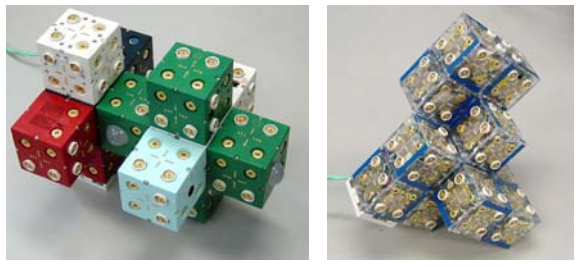
\includegraphics[width=.54\linewidth]{images/activecube}&
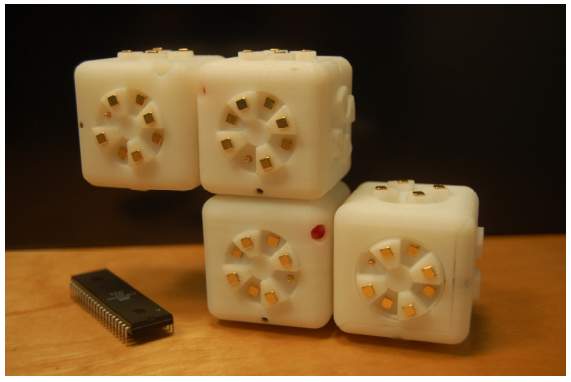
\includegraphics[width=.37\linewidth]{images/roblocks}
\end{array}$
\end{center}
\caption{Left: The ActiveCube system. Right: The Roblocks system.}
\label{fig:activecube}
\end{figure}

Related contributions focus more on the cognitive processes involved when
exploring embodied interfaces with children. Research on supporting creative
problem solving with children\cite{Bevans:2011:SCC:1979742.1979838}, arguing for
a kindergarten-influenced approach to creative
thinking\cite{Resnick:2007:IRN:1254960.1254961}, embodied approaches to
analyzing children's interactions with smart
objects\cite{Antle:2009:THE:1520340.1520612}, as well as the embodied design of
interfaces for introducing mathematical concepts to
kids\cite{Abrahamson:2011:TED:1999030.1999031} have shown a great degree of
correlation between physical interaction and learning in children.


\begin{figure}[ht]
\begin{center}$
\begin{array}{cc}
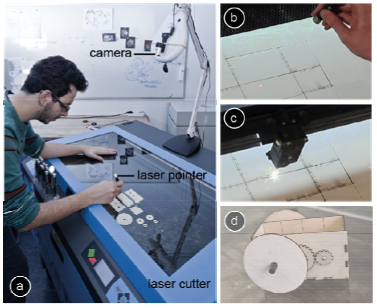
\includegraphics[width=.40\linewidth]{images/interactiveLaser}&
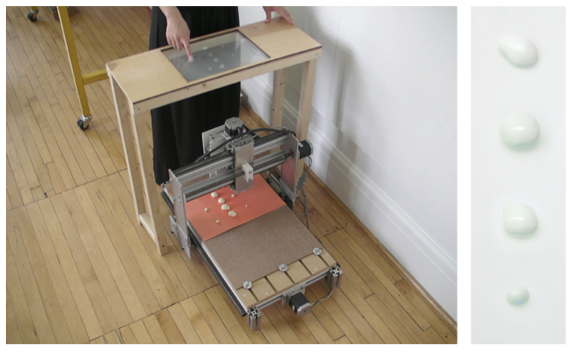
\includegraphics[width=.54\linewidth]{images/interactiveFab}
\end{array}$
\end{center}
\caption{Examples of interactive fabrication interfaces: Constructable (left)
allows users to control a laser cutter with a set of physical tools as opposed
to a pre-defined design file. Shaper (right), and interactive fabrication tool
using expanding polyurethane foam.}
\label{fig:kidcad}
\end{figure}



\begin{figure}[ht]
\begin{center}$
\begin{array}{cc}
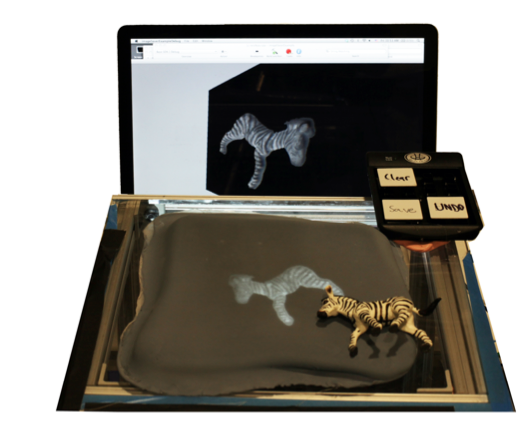
\includegraphics[width=.45\linewidth]{images/kidcad}&
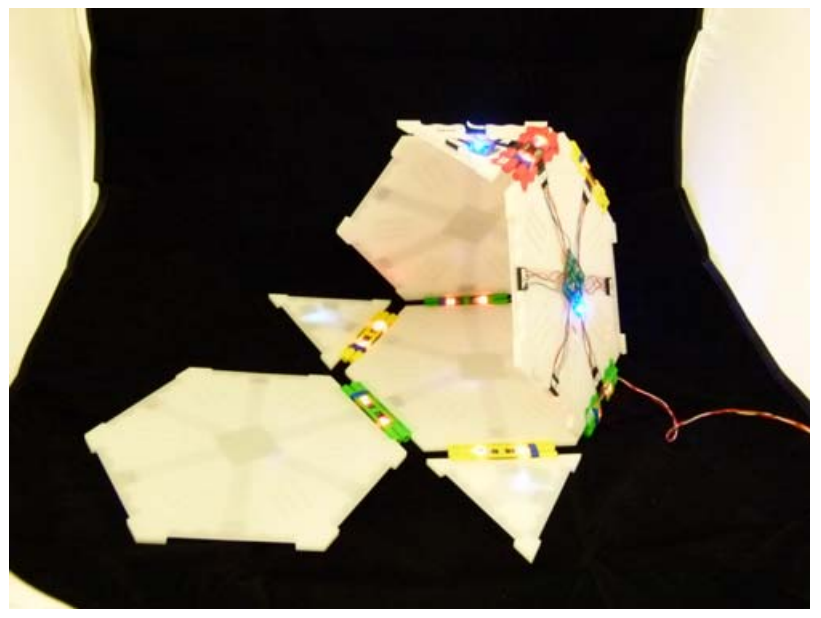
\includegraphics[width=.45\linewidth]{images/easigami}
\end{array}$
\end{center}
\caption{Left: The KidCAD interface showing a model Zebra and its 2.5D
impression on screen.
Right: The Easigami system, showing a series of connected polygonal faces with
smart-hinges and embedded electronics.}
\label{fig:kidcad}
\end{figure}

Yet so far, there have been few attempts to design embodied interfaces for
children that specifically address the growing presence and availability of
digital fabrication tools.
KidCAD\cite{Follmer:2012:KDR:2207676.2208403}, a deformable pad that captures
the 2.5D geometry of depressions made on the underside of the surface, was a
very promising idea in that it allowed very young children to take small objects
from their surroundings (or their hands) and `stamp' them into the pad - an
intuitive and satisfying experience. Unfortunately, the authors intentions to be
able to output the geometry to 3D printers has not yet manifested.
Easigami\cite{Huang:2012:EVC:2148131.2148143} is a set of interchangeable and
interlocking polyhedral faces with smart `hinges' that can reproduce the
morphology of a set of connected faces while connected to a computer. In
contrast, Easigami \emph{is} able to export this morphology to a
stereolithography file ready for 3D printing. There are several other interfaces
that deal with `interactive fabrication'\cite{Willis:2010:IFN:1935701.1935716};
devices that manipulate materials interactively based on various input from a
user, such as controlling a laser cutter with a laser pointer (instead of
through a CAD program)\cite{Mueller:2012:ICI:2380116.2380191}, or a wearable
device that takes in a CAD file and provides haptic feedback to make the
physical creation of the device by hand easier, even for a
non-fabricator\cite{Zoran:2013:FFD:2470654.2481361}.
These projects, as well as several others that deal specifically with digital
fabrication for laser
cutting\cite{Johnson:2012:SMS:2212776.2212390}\cite{Willis:2010:SSB:1709886.1709890},
are examples of the subset of tangible interfaces to which this work belongs -
namely, those concerned with providing a means to engage with digital
fabrication technologies in a more intuitive, embodied fashion. However, with
the exception of KidCAD and Easigami these designs are not made with children in
mind, nor do they cover the range of possibilities for child-friendly input
devices that focus on 3D-printing. Thus we argue that there is room for
exploration in this area, as well as a lineage that suggests meaningful results
may follow from the incorporation of tangible interfaces with embodied design.



% from IDC 2011
There are several strands of research that have strongly influenced the design
(and motivation) for the UCube. Perhaps the most fundamental of these is in the
area of "embodied mathematics"� that is, the notion that mathematical thinking
and learning are affected by, and perhaps grounded in, metaphors derived from
bodily experience. The most thorough and discursive (though largely theoretical)
discussion of these ideas is in the foundational text by Lakoff and Nu�ez
\cite{lakoff}:
the authors discuss physically-derived metaphors that underlie such essential
mathematical ideas as numbers, operations, and sets. Such notions of embodied
mathematics have�even before the Lakoff/Nu�ez text�played a role in discussions
of the development or instruction of mathematical ideas. The link between
physical experience and mathematical growth was a strong element, for instance,
in Montessori's work (see, e.g., \cite{hainstock1978essential}); much of the
motivation behind traditional mathematical ``manipulatives'' such as number rods
and balance beams can also be traced to this intellectual tradition. More
recently, theoretical discussions of embodied cognition have given rise to
fine-grained observations of the connections between bodily activity and
mathematical learning:
Goldin-Meadow\cite{goldin2005hearing}, for instance, describes a fascinating
line of research in which children's nonverbal gestures appear to both reflect
and, in some cases, anticipate their verbal understanding of concepts such as
conservation and ``inverse operations''.
Pedagogical research in embodied mathematics has, moreover, proceeded
hand-in-hand with the development of desktop, embedded, or portable
technological artifacts to support the link between bodily actions and
mathematical conceptualization. Papert's discussions of the Logo computer
language \cite{mindstorms} reveal this connection early in the history of
children's computing: Papert discussed, for example, the way in which the
program for a Logo circle resonated with children's bodily understanding of
moving in a circular path. More recently, Nemirovsky et al.
\cite{nemirovsky1998body} describe the use of a computer-based motion detector
system to assist children in the development of intuitions behind graphing;
Howison et al. \cite{howison2011mathematical} used a device based on a Wii
remote to assess children's understanding of ratio (the children attempt to move
their arms in a manner illustrating a target ratio); Bakker et al.
\cite{bakker2011moso} created a collection of handheld objects (``MoSo
Tangibles'') with embedded sensors to help children learn about musical ideas
via hand motions such as waving, squeezing (pressing hands together), and
shaking up and down, among others; Mickelson and Ju \cite{mickelson2011math} use
sophisticated video and projection equipment as the basis of activities through
which children can learn about mathematical ideas (e.g., symmetry, rotation
angles) via large- scale physical movements.
The development of the UCube follows within this tradition, in that the device
was created to enable children to specify and identify three-dimensional shapes
by hand motions (instead of, by contrast, using symbolic commands directed at a
two-dimensional screen display). At the same time, the UCube is not simply a
device for mathematical instruction, but is more generally a tool for
mathematical design. As noted at the outset of this paper, the intent of the
UCube is to enable youngsters not only to learn about but also to build
mathematical shapes.
Specifically, we see the device as part of a larger, burgeoning "technological
ecosystem" around the activity of three- dimensional printing. The first section
of this paper noted several prominent researchers who argue for the
democratization of this technology, and for its applications to education.
Indeed, exciting early work has been done in applying 3D printing to education
in fields such as architecture \cite{breen2003tangible}, solid geometry
\cite{hart2008procedural}, and mechanical design \cite{lipson20053}. The UCube
is designed so that it can be employed by younger students�younger, for
instance, than the typical (undergraduate-age) architecture student. At the same
time, we see no reason at all why the device could not be used by adult or
professional-level students�particularly if (as we anticipate) the device and
software are made more expressive or powerful in future iterations.
It should also be noted, along these lines, that our early pilot test experience
suggests a potentially fruitful use for the UCube as an assessment device for
children's spatial cognition. (The young subject who suggested that it could be
made into a "puzzle game" is anticipating our thoughts here!) A researcher
could, for instance, give children a pattern of lights and ask them to match
that pattern to one of a set of physical or pictorial solid representations; or
one might ask children to recreate a variety of physical solids (such as a
plastic prism or tetrahedron) by selecting the appropriate set of lights, and
note their development and difficulties in doing so. By using the UCube as an
experimental device in this fashion, one can position this work as part of a
tradition (dating back at least to Piaget \cite{piaget1967child}) in
understanding spatial thinking and its development (cf. also
\cite{newcombe2003making} for a more recent treatment of the subject).


%From IDC 2014 on paper-based electronics
Having shown several representative prototypes of our own work in paper
mechatronics, it is now worth situating that work in relation to that of other
researchers in this (still embryonic) field. The blending of traditional
papercrafts with emerging technology is in fact still a relatively novel
technique, but there is a remarkable community of researchers beginning to
explore this area. For us, a special debt is owed to Leah Buechley's High-Low
Technology group at the MIT Media Lab; that group first (to our knowledge)
introduced conductive ink and copper tape into paper-based projects. Early (c.
2008) use of conductive ink with microcontrollers on a paper substrate can be
found in \cite{buechley2009paints} and \cite{Eisenberg:2009:CPR:1551788.1551790}
with the development of paper-based Arduino processors and simple electronic
components (e.g. LEDs, toy motors, switches) that could be placed onto
conductive paint to form an electronic connection. This work culminated with a
paper application usually reserved for home remodeling: a ``living
wallpaper''\cite{Buechley2010} where passers-by could trigger light, movement,
and sound by interacting with different parts of the surface.



These early efforts in turn spawned developments that further refined the
expressive potential of paper-based electronics, infusing traditional
papercrafts with new elements and abilities. An electronic pop-up book by Qi and
Buechley\cite{Qi:2010:EPE:1709886.1709909} reimagined the traditional pop-up by
infusing each page with paper-friendly, interactive circuitry (e.g. by using
a copper tape circuit to power LEDs in a pop-up cityscape). Other projects in
this vein include techniques to animate origami structures through shape-memory alloy
(SMA)\cite{Qi2012}, using SMAs in the design and fabrication of
printable paper-based devices (e.g. speakers and lamps)\cite{Saul2010a},
storytelling and craft-making through electronically-enhanced storybooks and
workshops \cite{Jacoby2013a}\cite{Buechley2012}\cite{Sylla2012} and the use
of small microcontrollers incorporated into programmable
paper-based scupltures\cite{Mellis:2013:MMC:2460625.2460638}.

These efforts have focused on the creation of compellingc(either electronically
or digitally enhanced) papercrafts. As noted in the introduction, there are
numerous technological developments that, in combination, serve to accelerate
the development of paper mechatronics. For instance, Mueller et
al.\cite{Mueller:2012:ICI:2380116.2380191} describe the use of a laser cutter to
produce origami figures; Kawahara et al.\cite{Kawahara2013} describe how
inkjet-ready conductive ink can allow circuits to be printed easily and directly
onto paper; and Koizumi et al.\cite{Koizumi2010a} present a toolkit for wireless
control of moveable paper toys, Zhu et al.\cite{Zhu2011a} describe a method for
wireless power transfer for paper computing, and Coelho et al.\cite{Coelho2009}
have acheived the direct embedding of conductive components during the
papermaking process.

These last efforts are powerful examples of expanding techniques--they signal
the emergence of a new territory within which to explore paper-based electronics.
Our own prototypes are intended to continue this communal development of
techniques and examples, but there are several factors that distinguish our work
from that of other efforts. First, several of our own prototypes (e.g., PopCAD,
the bicycle rider, and the cherry blossom painting) may be seen as incorporating
paper elements as portions of larger, composite systems. PopCAD is a paper-based
input device; one might think of it as one early foothold in an unexplored
landscape of paper input devices for children's activities. The bicycle rider is
an artifact that combines a desktop computer screen with a paper model; again,
one could think of it as an exemplar of blending papercrafts with (e.g.)
high-resolution graphics, or one could imagine websites designed to work as
``background graphics'' for electronically-controlled paper constructions. The
cherry blossom painting is (in a sense) the ``flip side'' of PopCAD; whereas
PopCAD is a paper-based input device, the cherry blossom painting is a
paper-based display for output. And once more, one could take the example still
further: paper mechanisms or models could be moved or controlled as components
of extended output displays that combine physical and screen-based elements.

More generally, we see our prototypes as (still-early) pointers toward a new
genre of activities for children. In the final section, we turn our attention to
the mechatronic future of children's papercrafts.






